
\chapter{The Prompt Engineering Ontology: Requirements Specification}
\label{chapter:3_design}
This chapter details the design phase of the Prompt Engineering Ontology PEO, based on LOT, a state-of-the-art ontology engineering methodology.
Compared to other methodologies analysed, LOT is a recent methodology, introduced in 2022, and has been used in various projects such as the 'Ciudades Abiertas' project \cite{ciudad} for the construction of a set of ontologies used for sharing open data, and the BIMERR project \cite{bimerr}, in which ontologies for sustainable construction were developed \cite{bountouni2021bimerr}, among many others available on the LOT methodology website \footnote{https://lot.linkeddata.es/}.
LOT has not only been successfully applied in industrial projects, but also in the development of various research ontologies, as seen in Chapter~\ref{chapter:background}, as it provides a straightforward and iterative method for designing and developing ontologies.
Another reason for choosing LOT is its ease of learning, as it is inspired by the agile methodology in software development. The Linked Open Terms project not only provides very useful examples of ontologies to draw inspiration. LOT offers a Github repository \cite{lot_github} with all the necessary resources to be used in the specification of requirements.
This last aspect is very important because the main drawback of the other methodologies analysed is the lack of concrete guidelines and the relevant tools to use, tools that, when mentioned, are often obsolete or inaccessible.
This complicates the work of a developer who is approaching ontology engineering for the first time, as he needs to understand the fundamentals of the methodology but also figures out which development, validation, and testing software to use.
The LOT methodology, thanks not only to the numerous available resources but also to the clear and precise description of the method and the recent tools to be used, resolves these issues and simplifies the developer's work.
The LOT methodology has an inherently iterative nature and is oriented towards the publication of ontologies according to the FAIR principles \cite{fair_eu}, including specific recommendations, tips and potential
tools that can be helpful to ontology developers.
Moreover, the methodology extends the state-of-art methodologies like NeOn and Methontology with a modern approach.

The LOT methodology was preferred over recently introduced techniques that involve the use of LLMs.
Although these techniques automate the process, they are computationally expensive and require numerous checks to verify the syntactic and semantic correctness of the produced artifact.
Another downside is the lack of actual ontology projects implemented using LLMs, as these are very recent techniques that have not been tested on real projects but only on experimental cases.
In the following sections, the application of the LOT methodology, methodology that has been discussed in Chapter \ref{chapter:background}, to the design and implementation of PEO will be described, following the workflow outlined and described in the background chapter.
\section{Use Case Specification}
The LOT methodology includes six mandatory phases (plus one optional) in the ontology requirements specification.
At the end of each phase, a document is produced containing the analysed aspect of the specifications, as shown in the following figure \ref{fig:13}:
\begin{figure}[H]
    \centering
    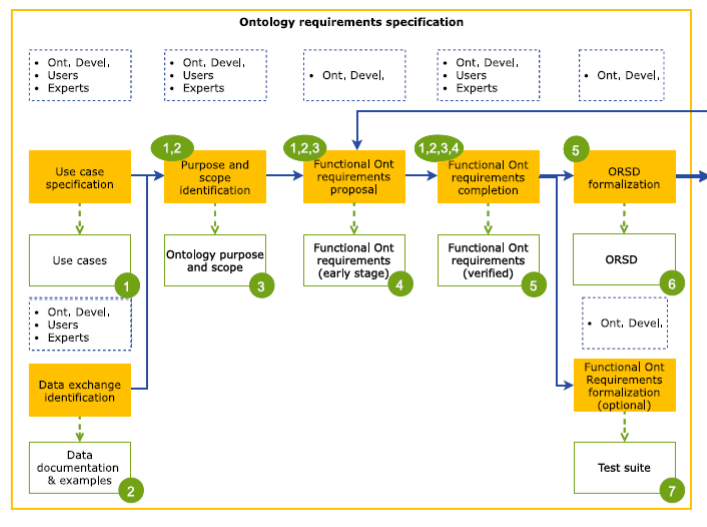
\includegraphics[width=0.9\linewidth]{Figures/fig_13.PNG}
    \caption{Ontology requirements specification workflow}
    \label{fig:13}
\end{figure}
In detail the phases are the following:
\begin{enumerate}
    \item Use case specification
    \item Data exchange identification
    \item Purpose and scope identification
    \item Functional ontology requirements proposal
    \item Functional ontology requirements completion
    \item ORSD formalization 
    \item Functional ontology requirements formalization (optional)
\end{enumerate}
The first step in the design of PEO is the use case specification, this phase involves domain experts, ontology developers and users and it has the goal to imagine and specify how the ontology can be used in real life by real users.
Taking into account the domain, the possible use and the possible users we decided to specify ten use cases.
Each use case has a name, a description, a list of actors and a flow.
\paragraph{Use case 1}
\begin{itemize}
    \item Name: Optimizing LLM Responses
    \item Description: Researchers use PEO to design optimized prompts that improve LLM response quality.
    \item Actors: Researcher, PEO, LLM.
    \item Flow: The researcher uses the ontology to identify appropriate prompts for different types of tasks creating a set of selected prompts. Selected prompts are given as input to the LLM and responses are evaluated according to specific metrics on consistency, completeness and quality decided by the researcher.
\end{itemize}
\paragraph{Use case 2}
\begin{itemize}
    \item Name: Bias analysis
    \item Description: Researchers use PEO to generate responses and detect bias in the considered LLMs.
    \item Actors: Researcher, PEO, LLMs
    \item Flow: The researcher uses the ontology to generate prompts on sensitive topics (e.g., gender, ethnicity) and prompts are tested on one or more LLMs. Responses are collected using bias and fairness metrics and results are collected in order to improve prompts and considered models. 
\end{itemize}

\paragraph{Use case 3}
\begin{itemize}
    \item Name: Code generation
    \item Description: Developers use prompt engineering techniques applied to a chosen LLM to generate source code in a specific programming language for a specific task.
    \item Actors: Developers, PEO, LLM
    \item Flow: The developer is working on an Android application written in Java and needs code to control the actions on a button. Using the ontology, he chooses the most appropriate prompt engineering technique and applies it to the creation of the prompt to a large language model of his choice,  resulting in Java code as output. The code is tested and integrated into the application. 
\end{itemize}

\paragraph{Use case 4}
\begin{itemize}
    \item Name: Prompt engineering lesson
    \item Description: The teacher uses PEO to teach prompt engineering techniques exploring different techniques and prompt described.
    \item Actors: Teacher, students, PEO. 
    \item Flow: The teacher opens the ontology and shows with proper explanation different prompt engineering techniques represented in the ontology.
\end{itemize}

\paragraph{Use case 5}
\begin{itemize}
    \item Name: LLMs lesson
    \item Description: The teacher uses PEO to teach the different LLMs available.
    \item Actors: Teacher, students, PEO.
    \item Flow: The teacher opens the ontology and shows with proper explanation different LLMs represented in the ontology. 
\end{itemize}
\paragraph{Use case 6}
\begin{itemize}
    \item Name: Social media content creation
    \item Description: The content creator uses PEO to generate prompts that optimize the creation of articles, social media posts and other textual content.
    \item Actors:  Content creator, PEO, LLM
    \item Flow: The content creator opens the ontology and chooses the appropriate technique in order to generate text for a post on social media using a specific large language model. The content creator adapts the response according to his target.
\end{itemize}

\paragraph{Use case 7}
\begin{itemize}
    \item Name: Image generation
    \item Description: The content creator uses PEO to create a prompt to be given as input to a specific large language model capable of generating an image.
    \item Actors: Content creator, PEO, LLM.
    \item Flow: The content creator wants to create an AI-generated image for a video and he uses the ontology to choose the best large language models able to generate image, he chooses the prompt engineering technique to create the prompt in order to generate image. He watches the output and he continues to use the ontology to generate prompts in order to refine the image.
\end{itemize}

\paragraph{Use case 8}
\begin{itemize}
    \item Name: Prompt engineering experiments
    \item Description: Students use PEO to explore and create effective prompts to improve language model responses.
    \item Actors: Students, PEO, LLM.
    \item Flow: Students explore the ontology in order to understand different prompting techniques applying them to a chosen large language model.
\end{itemize}

\paragraph{Use case 9}
\begin{itemize}
    \item Name: Large language models learning
    \item Description: Students use PEO to learn different types of large language models.
    \item Actors: Students, PEO
    \item Flow: Students explore different large language models represented in the ontology and the relations among them, learning all the features of each large language model.
\end{itemize}

\paragraph{Use case 10}
\begin{itemize}
    \item Name: Explanation computer science topics
    \item Description: Student wants to generate a prompt using PEO in order to explain a computer science topic.
    \item Actors: Student, PEO, LLM
    \item Flow: The student uses the ontology to choose the most appropriate prompt engineering technique in order to generate using large language models. The student reads the obtained LLM response and can create a new prompt using another technique represented in the ontology.
\end{itemize}

\section{Data Exchange Identification}
The goal of the data exchange identification activity is to provide the necessary documentation about the domain to be modelled.
Essentially, this phase involves gathering heterogeneous sources of information, such as scientific papers, websites, datasets, and similar existing ontologies.
Since LOT does not provide a clear indication on how to represent this documentation, we simply noted the URLs of the gathered resources.
The following list of papers was chosen as a source for PEO:

\begin{itemize}
\item A Systematic Survey of Prompt Engineering in Large Language Models: Techniques and Applications \cite{sahoo2024systematic}

\item Pre-train, Prompt, and Predict: A Systematic Survey of Prompting Methods in Natural Language Processing \cite{liu2023pre}

\item A Survey of Large Language Models \cite{zhao2023survey}

\item Investigating Prompt Engineering in Diffusion
Models \cite{witteveen2022investigating}

\item A Survey on Large Language Models: Applications,
Challenges, Limitations, and Practical Usage \cite{hadi2023survey}

\item Large Language Models: A Survey \cite{minaee2024large}
\end{itemize}
The list of website chosen is the following:
\begin{itemize}
    \item \href{https://www.promptingguide.ai/}{Prompting Guide}
    
    \item \href{https://github.com/Hannibal046/Awesome-LLM}{Awesome-LLM}

    \item \href{https://llmmodels.org/}{List of LLMs}

    \item \href{https://learnprompting.org/}{Learn prompting}
\end{itemize}
We decided to select these research papers and websites to build a well-structured and comprehensive ontology for prompt engineering and large language models. The academic papers provide in-depth analyses of prompting techniques, their applications, and the evolution of LLMs, offering a strong theoretical foundation. Meanwhile, the chosen websites serve as practical resources, curating up-to-date information on LLM architectures, prompting strategies and real-world use cases. 


\section{Purpose and Scope Identification}
From use cases and the domain documentation provided in the data exchange identification task, in this phase there is the specification of the purpose: what is the objective of PEO and the specification of the scope of the ontology: what it is going to be represented in the ontology.
The objective of PEO is to formalize knowledge about the creation and various types of prompts for the different LLMs available by making it accessible to both experienced and less experienced users.
PEO aims at covering the following scope:
\begin{itemize}
    \item LLMs available to users
    \item Prompt engineering techniques
    \item Task that can be solved using a LLM
    \item Examples of prompts specific to the LLM
\end{itemize}
In general, the goal of the project and the ontology is to create a resource accessible to everyone on a recently introduced topic, for which there are not many available resources.
This resource aims to support not only the learning but also the application of prompt engineering techniques and LLMs.

\section{Functional Ontology Requirements Specification}
In LOT methodology there are three possible ways to specify the requirements: CQs, natural language statements and tabular information containing concepts, relations, and attributes.
As seen in Chapter~\ref{chapter:2_background}, competency questions are widely used in ontology engineering and allow for clearly expressing the functional requirements of an ontology.
In the case of PEO, based on the use cases and the purpose and scope identification described earlier, we have identified sixteen CQs:
\begin{itemize}
    \item CQ1: What is prompt engineering?

    \item CQ2: What is a prompt?

    \item CQ3: What are prompting techniques?

    \item CQ4: What are image prompting techniques?

    \item CQ5: What are code prompting techniques?

    \item CQ6: Which task does a prompt solve?

    \item CQ7: Which prompts are generated using a prompting technique?

    \item CQ8: What are the responses that follow each prompt?

    \item CQ9: What are possible tasks?

    \item CQ10: Which tasks are related to the text?

    \item CQ11: What is a chat?

    \item CQ12: What is a large language model?

    \item CQ13: What types of large language models are available?

    \item CQ14: What are large language models architectures?

    \item CQ15: What are large language models capabilities?

    \item CQ16: What companies develop large language models?
\end{itemize}

CQs are saved into an excel file, the template is available in the official Github repository \footnote{https://github.com/oeg-upm/LOT-resources}.
The Excel file not only contains the CQs, but also specifies for each one: the identifier, the domain, the answer, the status (Proposed, Accepted, Rejected, Pending, Deprecated), comments, and priority (high, medium, and low).
All the CQs have a high priority, as they form the foundation of PEO, covering both prompt engineering and LLMs.

\section{Document Formalization}
The final step in the specification of ontology requirements is the writing of the ORSD, a document that gathers the main information defined in the previous phase, namely the purpose and scope of the ontology, the use cases, the functional requirements (expressed through CQs), and the non-functional requirements.
First introduced by the NeOn methodology, which we discussed in the previous chapter, the writing of the ORSD follows a specific sequence of tasks to ensure its correctness and completeness.
The workflow \cite{suarez2009write} involves a sequence of eight tasks, starting from ontological needs: 
\begin{enumerate}
    \item Identify purpose, scope and implementation language.
    \item Identify intended end-users
    \item Identify intended uses
    \item Identify requirements
    \item Group requirements
    \item Validate the set of requirements
    \item Prioritize requirements
    \item Extract terminology and its frequency
\end{enumerate}
LOT adopts (a customized version of) the ORSD introduced by NeOn.
Unlike NeOn, it does not consider the "user" field as mandatory, and the glossary of terms is built starting from the competency questions.
In writing the ORSD for PEO, the  template from the official LOT repository \footnote{https://github.com/oeg-upm/LOT-resources/tree/master/templates\%20for\%20ORSD} was used. 
In the document, the information obtained in the previous phases has been included, namely purpose and scope identification and ontology requirements in the form of CQs.
Additionally, further information that emerged during the requirements gathering phase has also been included:
\begin{itemize}
    \item Implementation language 
    \item Intended End-Users 
    \item Intended Uses
    \item Non-Functional Requirements
\end{itemize}
In detail, the implementation language is OWL using the Protegé software\cite{protege_sw}, an open-source popular software released by Stanford University.
As seen in the use cases, the intended end-users of PEO are:
\begin{itemize}
    \item Researchers in the field of AI using LLMs for research purpose.
    \item Software engineers and developers.
    \item Educators and trainers teaching students or professionals about AI and prompt engineering, using the ontology as a learning and instructional tool.
    \item Content Creators using LLMs for generating content.
    \item Undergraduate and high school students learning about AI, LLMs and prompt engineering, using the ontology to understand core concepts and experiment with language models.
\end{itemize}
Starting from the use cases, it is possible to easily deduce the intended uses:
\begin{itemize}
    \item Prompt generation
    \item LLMs learning
    \item Prompt engineering learning
    \item Prompt generation for a specific task
\end{itemize}
Regarding non-functional requirements, i.e., the characteristics, qualities and general aspects not related to the ontology content that the ontology should satisfy, we have identified three non-functional requirements:
\begin{itemize}
    \item NFR1: The ontology must be published on main ontology repositories
    \item NFR2: The ontology must have exhaustive documentation.
    \item NFR3: The ontology must be easy to update.
\end{itemize}
Those non-functional requirements match with the desired properties of PEO, since the ontology has to be accessible for everyone by publishing on main ontology repositories. The documentation  must be exhaustive and clear for users to understand the content of the ontology and it could be useful for possible updates.




